\subsection{Difference between the Radiation Transfer Equation and Reinhart Equation (9)}

\subsubsection{Radiation Transfer Equation}

\begin{align}
	\dfrac{d I(\lambda)}{ds} = - I(\lambda) \kappa(\lambda)
\end{align}
\begin{align}
	\dfrac{I_{abs}}{I_0} = \int_{\lambda_1}^{\lambda_2} \left(1 - \exp(-\kappa(\lambda) z)\right) d \lambda
\end{align}

\subsubsection{Reinhart Equation (9)}

\begin{align}
	\dfrac{I_{abs}}{I_0} = \sum_i (1 - \exp(-\kappa_i z)) \Delta \lambda_i
\end{align}

\subsubsection{Simple Model}

Two partially overlapping lines with rectangle shaped line shapes:
\begin{figure}[ht]
	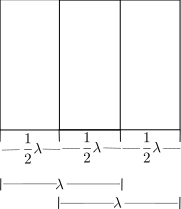
\includegraphics[width=6cm]{figures/overlappinglines2.png}
	\caption{Two overlapping lines with rectangle line shape functions}
	\label{fig:overlappinglines}
\end{figure}

Reinhart:
\begin{align}
	\Delta J_1 &= \left(1 - \exp( - \kappa_1 z)\right) \Delta \lambda \\
	\Delta J_2 &= \left(1 - \exp( - \kappa_2 z)\right) \Delta \lambda 
\end{align}
\begin{align}
	A = \dfrac{\Delta J_1 + \Delta J_2}{\Delta \lambda} = \left(1 - \exp( - \kappa_1 z)\right) + \left(1 - \exp( - \kappa_2 z)\right)
\end{align}
Radiation transfer solution :
\begin{align}
	\Delta I_1 &= \left(1 - \exp( - \kappa_1 z)\right) \dfrac{\Delta \lambda}{2} \\
	\Delta I_2 &=  \left(1 - \exp( - \kappa_2 z)\right) \dfrac{\Delta \lambda}{2} \\
	\Delta I_{12} &= \left(1 - \exp( - \kappa_1 z - \kappa_2 z)\right) \dfrac{\Delta \lambda}{2}
\end{align}
\begin{align}
	B = \dfrac{\Delta I_1 + \Delta I_2 + \Delta I_{12}}{I_0 \Delta \lambda} =
			& \dfrac{1}{2} \left(1 - \exp( - \kappa_1 z)\right) +  \\
			& \dfrac{1}{2} \left(1 - \exp( - \kappa_2 z)\right) + \\ 
			& \dfrac{1}{2} \left(1 - \exp( - \kappa_1 z - \kappa_2 z)\right) 
\end{align}
The difference is:
\begin{align}
	2(A - B) &= \left(1 - \exp( - \kappa_1 z)\right) + \left(1 - \exp( - \kappa_2 z)\right) -
	\left(1 - \exp( - \kappa_1 z - \kappa_2 z\right) \\
	         &= 1  + \exp(- \kappa_1 z - \kappa_2 z) - \exp( - \kappa_1 z) - \exp( - \kappa_2 z)
\end{align}
In case of $\kappa_1 \gg 1$ and $\kappa_2 \gg 1$ this yields: 
\begin{align}
	(\Delta J_1 + \Delta J_2) - (\Delta I_1 + \Delta I_2 + \Delta I_{12})=
	I_0 \dfrac{\Delta \lambda}{2}
\end{align}
That means the absorption of the overlapping region is counted twice.